\chapter{APPLICATIONS}
\label{chap:applications}

Previous chapters focused more on various technical aspects of co-channel speech and less on integrating the proposed techniques with other applications. 
This chapter highlights collaborative studies that address co-channel speech analysis for two problems: word-count estimation and in-vehicle speech pertaining to driver safety systems.\footnote{Word-count estimation in co-channel speech is a collaboration between myself, Ali Ziaei, Abhijheet Sangwan, and my advisor Prof. John Hansen. At the time of the study, Ali Ziaei was a fellow PhD student at CRSS, Abhijeet Sangwan was (and currently still remains) a research professor in the department of Electrical Engineering at UT-Dallas. 

In-vehicle speech analysis studies are a collaboration with Amardeep Sathyanarayanan, Omid Sadjadi, and Prof. John Hansen. Amardeep and Omid were both PhD students at CRSS during the time of these studies.} 
I consider these studies a driving force during my work as a PhD student, since research without outside stimulus can sometimes be mundane and out of touch. 
Collaborative studies, on the other hand, open up room for discussion and often lead to constructive feedback. 
Each of the studies presented in this chapter have led to major advancements in this dissertation. 

The contribution of this chapter is:
\begin{itemize}
	\item use overlap detection to improve word-count estimation in real environment noise conditions. 
	\item use overlap detection to predict competitiveness in conversations in in-vehicle speech analysis. 
\end{itemize}
Prior to the study on word-count-estimation, the main overlap detection algorithm developed for this dissertation was Gammatone sub-band frequency modulation (GSFM; see Sect.~\ref{sec:ch2_GSFM} in Chapter~\ref{chapter:front-end}). As we have learned, GSFM is highly susceptible to noisy conditions. 
This observation was made while evaluating overlapped speech detection in Prof-life-log data, a dataset with various types and amounts of noise~\cite{ziaei2013prof}. 
Pyknograms were the solution to a long-lasting effort of developing a robust overlap detection method for noisy conditions (see Sect.~\ref{sec:ch2_Pykno}~and~\ref{sec:ch2_Pykno_vs_GSFM} in Chapter~\ref{chapter:front-end}). 

In-vehicle speech analysis contributed to a significant novelty in this dissertation's perspective in addressing co-channel speech (in terms of distinguishing co-channel speech from overlap). 
Prior to the collaborative study on in-vehicle speech, the sole focus of this dissertation was on examining overlapped speech. 
It was during this project that the importance of other conversational traits, such as turn-takings and speaker response time, became more visible and prompted further investigation. 

The remainder of this chapter provides a brief description of word-count estimation, Sect.~\ref{sec:wce_cch}, and in-vehicle driver safety systems, Sect.~\ref{sec:invehicle}. 


\section{Word-Count Estimation in Co-channel Speech}
\label{sec:wce_cch}
The ability to estimate the number of words spoken by an individual over a certain period of time is valuable in second language acquisition, health-care, and assessing language development. 
Word-count values are also useful in the analysis of massive audio data, such as the Prof-life-log corpus~\cite{ziaei2013prof}. 
Prof-life-log is a speech corpus that contains long durations of audio recordings. In this collection, the primary speaker wears a portable LENA recording device~\cite{lena_device} throughout a work day. 
Although the primary speaker is always the same individual, he frequently interacts with different people. 
An estimate of the primary speaker's speech activity (i.e. word-count) facilitates analyses that predict the level of productivity and helps determine areas in the recording that are more ``valuable'' for further processing. 
The proposed word-count estimator in this study is tested on long duration files from the Prof-Life-Log corpus. 

Establishing a robust automatic framework to achieve high accuracy is non-trivial in realistic scenarios due to various factors such as different conversation styles or types of noise that appear in audio recordings, especially in multi-party conversations (i.e., co-channel speech). 
This section proposes to use overlap detection to estimate the likelihood of overlapping speech in a given audio file in the presence of environment noise. 
The resulting overlap information is embedded into a word-count estimator, which uses a linear minimum mean square estimator (LMMSE) to predict the number of words from syllable rates, which are easier to detect using only acoustic information. 
Figure~\ref{fig:ch6_wce_system_overview} shows an overview of the proposed word-count estimator. 
The overlap detection system acts as an augmented module in the system, similarly to how speech activity detection removes silence for the word-count estimation (WCE) system. 

\begin{figure}[t!]
	\centering
	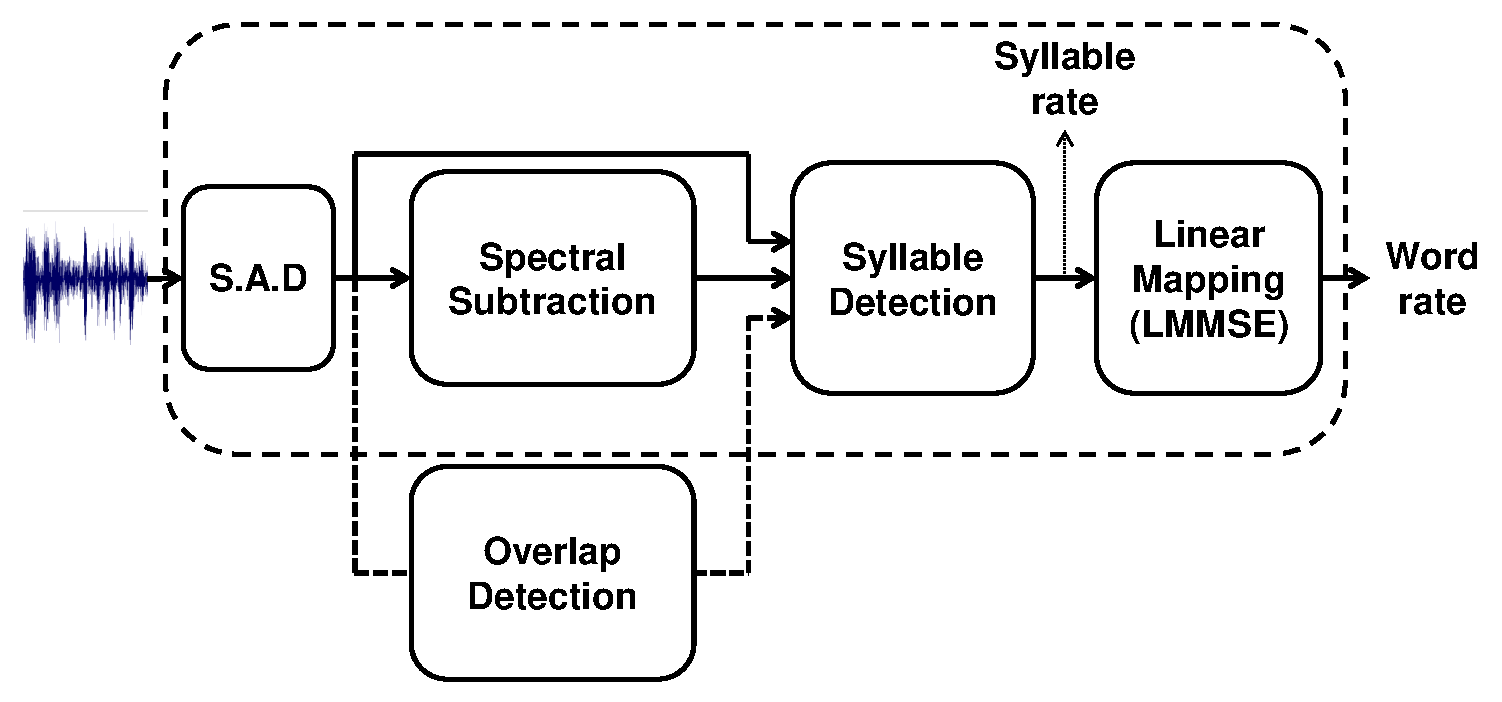
\includegraphics[height = 2.8in, width=1\textwidth]{figures/wce_ovl_SLT2014_systemconfig_figur-crop}
	\vspace{-3mm}
	\caption{Word-count estimation system configuration. The overlap detection system is shown as an addition to the original system.}
	\label{fig:ch6_wce_system_overview}
\end{figure}

\subsection{Word-count estimation}
\label{sec:wce}
The word-count estimator is adopted from previous studies~\cite{IS14_wce}, which estimate the number of words per unit time by applying a linear transformation to the syllable rate. 
Syllable rates are calculated based on a modified version of the {\it mrate} algorithm~\cite{Wang_slbl} using acoustic characteristics of the signal: pitch, smoothed spectrogram. 
This algorithm detects the location of syllables in a given speech segment. 
The number of detected syllables per unit time are used to calculate syllable rates throughout the audio. 
As~\cite{IS14_wce} show, the help of alinear minimum mean square estimator (LMMSE) can generate linear coefficients that map syllable rates to the number of words per unit time, as shown below: 
\begin{equation}
\label{eq:lmmse_wce}
{\tilde {\bf a}} = argmin_{\bf a} \Big\{\frac{1}{N}\sum_{\bf a}\big(W_r(n)-{\bf a}S_r(n)\big)^2\Big\},
\vspace{-1mm}
\end{equation}
where $W_r(.)$ and $S_r(.)$ are the word-count and syllable rates at any given time, respectively. 
$n$ indicates the index of a given time segment and $N$ is the total number of segments used to train the linear transformation parameter, ${\tilde {\bf a}}$. 
The transformation parameter, ${\tilde {\bf a}}$, is a vector comprised of a bias factor and a linear coefficient. 
In cases where the bias factor is non-zero, $S_r(n)$ is replaced by $\big[S_r(n) \hspace{2mm} 1\big]^T$. 
The linear transformation parameter(s) can be trained using manually transcribed background conversational data. 
For this study, we rely on a subset of Prof-Life-Log data that has been transcribed for word-counts. 

In~\cite{IS14_wce}, higher accuracy is obtained by introducing speech activity detection (SAD)~\cite{sadjadi2013unsupervised} and spectral subtraction to the front-end of the WCE. 
SAD reduces false-alarms by omitting non-speech regions, a decrease which helps avoid detection errors made by the syllable detector. 
Spectral subtraction enhances speech regions~\cite{boll1979spectralSubtraction}, allowing the syllable detector to identify voiced regions more accurately. 
None of these techniques, however, are able to address the issue of overlapped speech. 
Therefore, the novelty in this study is to use overlap detection as an additional layer of data pruning to reduce false alarms. 

An estimation of the location and amount of overlapped speech in a given speech segment can be combined with SAD labels to supply an additional layer of data pruning before syllable detection. 
Overlap detection is fed to the syllable detector as additional information (see Fig.~\ref{fig:ch6_wce_system_overview}).  
First, SAD is performed on the raw data to detect speech locations. 
From SAD labels, non-speech regions are used to estimate the noise level in each short segment and submitted to the spectral subtraction algorithm. 
Speech-only segments are passed to the syllable detector after applying spectral subtraction. 
Finally, syllable rates (calculated by dividing the number of syllables by the segment length) are transformed into word-count rates using LMMSE coefficients. 
In our proposed system, overlap detection outputs are combined with SAD results, to provide an extra layer of data pruning. 

The overlap detection algorithm used in this framework is based on Pyknograms, which are described in Chapter~\ref{chapter:front-end}. 
Pyknograms were chosen here as a robust solution to the highly noisy data in Prof-life-log. 
In Pyknograms, non-resonant speech is emphasized over background noise and unvoiced speech. 
This allows improved performance in noisy conditions, while simultaneously improving syllable detection, due to the high correlation between voiced speech and syllables. 

\begin{table}[b!]
	\centering
	\renewcommand{\tabcolsep}{2.5 mm}
	\renewcommand{\arraystretch}{1.3}
	\vspace{0mm}
	%\vspace{1mm}
	\caption {WCE performance in Prof-Life-Log with respect to overlapped speech.}
	\label{tab:wce_ovl}
	\vspace{2mm}
	\begin{tabular}{p{0.8cm}*{6}{c}}
		\bf $\frac{minimum\hspace{1mm} mean \hspace{1mm} square \hspace{1mm} Error}{\# of words}$\\ \hline \hline
		overlaps & NOT&\hspace{-7mm}removed	&  &     &    5.71\% \\ 
		overlaps&\hspace{1mm} removed	&		&	&     &    \bf3.69\% \\ \hline
	\end{tabular}
	\vspace{-1mm}
\end{table} 

Word rates are extracted from 5 days of prof-life-log recordings. 
Each day contains roughly 6 to 8 hours of audio, labeled to include the transcriptions of the primary speaker's speech, speaker labels (primary vs. secondary), and the type of environment in which the recordings take place. 
We have mostly concentrated on environments that are more likely to contain overlapped speech, such as multi-party meetings and conferences.
The sampling frequency from the LENA device is $44.1kHz$, which we have down-sampled to $8kHz$. Table~\ref{tab:wce_ovl} shows over $35\%$ improvement in relative mean square error after removing overlapped regions. 


\newpage
\section{In-vehicle Conversation Analysis}
\label{sec:invehicle}
Many in-vehicle conversations are beneficial in keeping drivers alert and active, however there are also instances where a competitive conversation may adversely influence driving performance. 
Identifying such scenarios can improve vehicle safety systems by fusing the knowledge obtained from conversational speech analysis and vehicle dynamic signals. 
This section briefly describes how smart portable devices can be incorporated to create a unified platform and record in-vehicle speech as well as vehicle dynamic signals required to evaluate driving performance. 
This study shows that turn-takings and overlapped speech segments, as conversational speech cues, under certain conditions deviate from normal driving patterns. 

Auditory based distraction caused by in-vehicle conversations is difficult to investigate. The main issue being that not all speech activity is considered distractive to drivers. 
The study in \cite{ESPA} used speech activity detection to track the impact of any speech activity on driving performance. 
The conclusion being that although some impact is observed, driving performance is highly affected by the type of conversation. 
In this study, we further investigate the possible consequences of drivers' involvement in \emph{competitive} conversations while driving. 
It is expected that active engagement conversations results in deviations from usual driving patterns, which are identified through the analysis of different driving maneuvers. 

\subsection{System Description}
\label{sec:system_description}
\vspace{3mm}
Performing certain secondary tasks while driving is likely to adherently impact driving performance. 
Some tasks are inevitable or difficult to restrict, such as controlling the navigation system. 
However, other secondary tasks such as engaging in a conversation with other passengers or cell-phone conversations can be controlled if they are determined to compromise driving performance. 
This sections shows a feedback system which not only evaluates variations in driving performance but also helps mitigate the influence of in-vehicle speech if it is found to adversely influencing the driving performance (see Figure~\ref{fig:ch6_system_description_fig}). 
There are two separate subsystems in the proposed framework. 
The first subsystem evaluates the driving performance by identifying maneuvers and then comparing them with the driver's regular driving patterns. 
If a maneuver is recognized as ``abnormal'', the driver's in-vehicle speech involvement is monitored to see whether that is the cause for unusual driving behavior. 

\begin{figure}[h]	
	\centering
	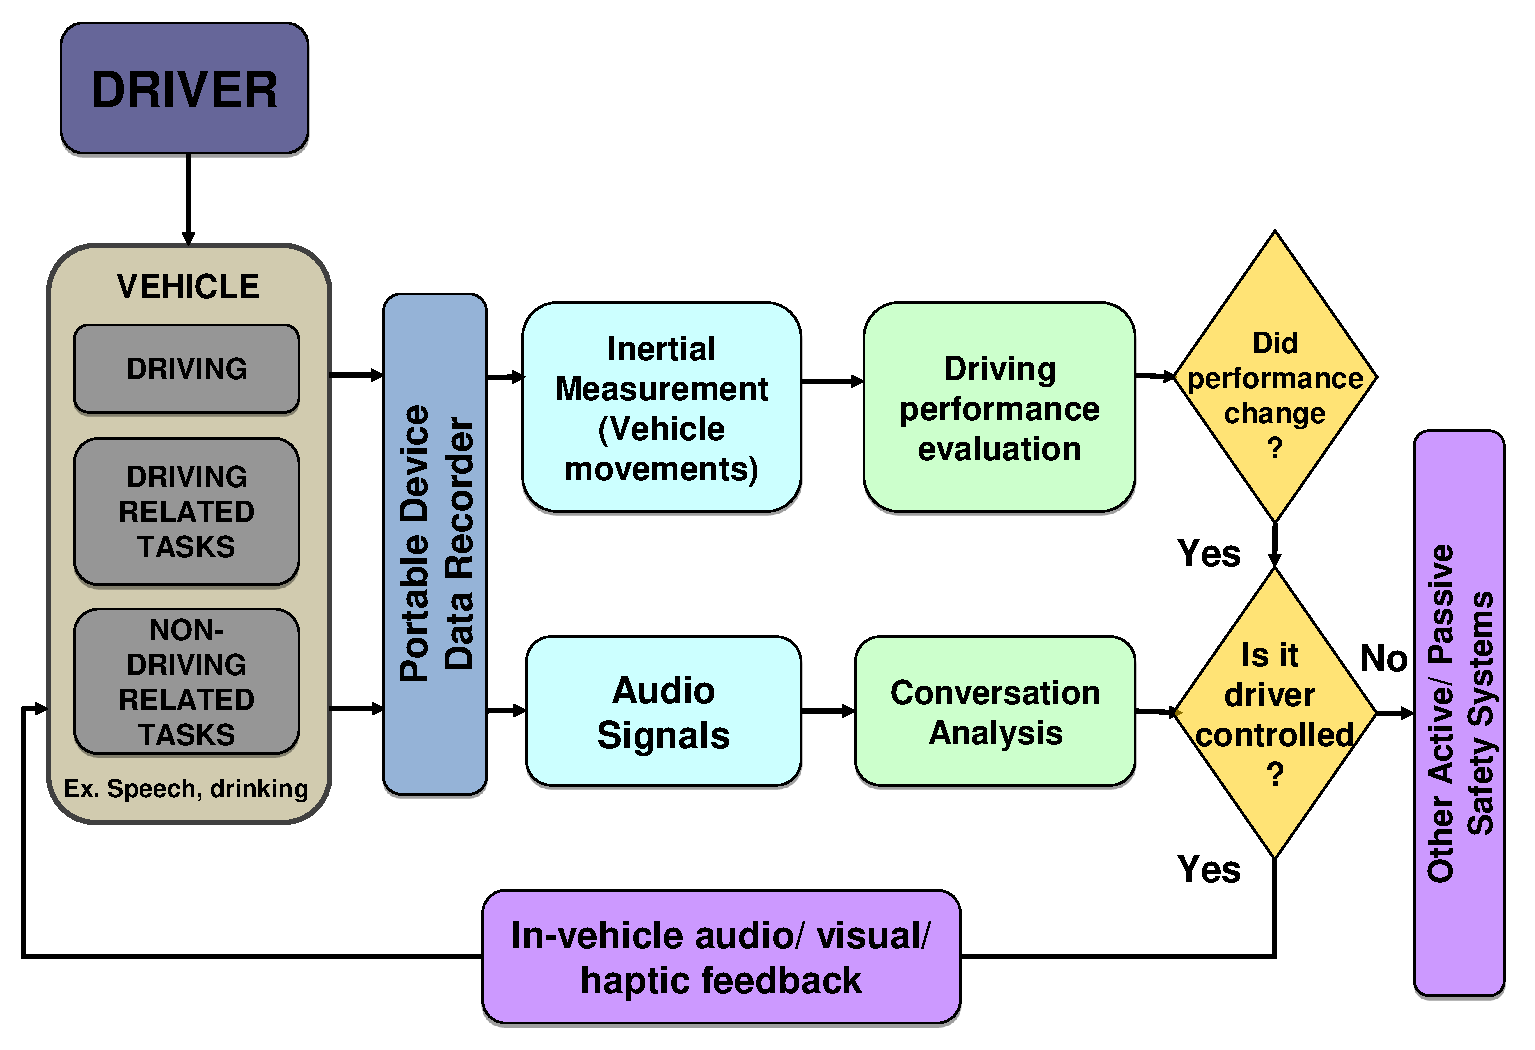
\includegraphics[width=\linewidth]{figures/system_description-crop}
	\caption {System description}
	\label{fig:ch6_system_description_fig}
\end{figure}

The second subsystem evaluates the driver's involvement in conversations. 
An addition to previous studies on in-vehicle speech~\cite{ESPA} is that rather than considering any in-vehicle speech activity, the emphasis here is on the driver's involvement in conversations. 
This involvement is analyzed by measuring the amount of overlapped speech segments as well as turn-taking rates during conversations. 
One of our objectives was to demonstrate that these two metrics are reliable indicators of the driver's focus on speaking as opposed to the primary task, which is driving. 
If in-vehicle speech activity is identified to adversely impact the driver's performance, it can be controlled passively by providing an initial warning feedback to the driver and/or co-passengers to halt the conversation until the vehicle state returns back to normal. 
Monitoring driving performance continues and any secondary tasks performed by the driver, other than those essential to driving, could be sequentially cut off. 
The uniqueness of this system is the ability to identify driving performance variations and isolate the source of distraction. 

The technical details of the driving evaluation system falls beyond the scope of this dissertation. 
For the curious reader, it suffices to know that performance is measured by statistically modeling driving maneuvers using vehicle dynamic signals (e.g., steering wheel angle, speed, acceleration)~\cite{sathyanarayana2013belt}. 
Maneuvers form the basic building blocks of driving routes, hence analyzing them can be employed as a key component in understanding driving performance. 
Variations in driving performance can be recorded by observing how each maneuver is executed and comparing the characteristics of maneuvers that fall under the same category. 

\subsection{Conversation Analysis}
\label{sec:conversation_analysis}
As mentioned in Section~\ref{sec:system_description}, the purpose of utilizing audio data is to analyze the conversation taken place in the vehicle and determine whether it is causing driver distraction. 
We speculate that the level of competitiveness in a conversation should correlate with driving performance. 
In order to measure competitiveness in a conversation, two features are utilized. 
The first is the turn-taking rate. 
An increase in the number of turn takings per time unit can imply that speakers are taking interest in the conversation. 
Additionally, the amount of overlapped speech is considered a potential competitiveness feature~\cite{Schegloff}. 

By now the readers are likely familiar with overlap detection algorithms, but turn-taking has not been covered in this thesis. 
Although there are more sophisticated ways of estimating turn-takings rates in a conversation (using speaker diarization). 
This study uses speech activity detection (SAD) to detect start and end-points of active speech regions in a conversation. 
The start-points are labeled as the triggering points of a turn in the conversation. 
Since this definition for turn taking may not always imply that both speakers are involved in a conversation, for example in instances when one of the speakers pauses in between sentences, the amount of overlapped speech in regions with a high turn taking rate is used to assure that both speakers are involved. 


\vspace{3mm}
\section{Data Description}
\label{sec:data_description}
Since this study focuses on understanding the influence of in-vehicle speech on the driver, care should be taken to minimize influence from other modalities on the driver.  
An experimental setup was conducted that allowed drivers operate the UTDrive vehicle under real-traffic conditions~\cite{pongtep2007utdrive}. 
The data was collected under similar weather and traffic conditions for all drivers and the route consisted of residential areas and highways and took place in an average of twenty minutes per session. 
In the past few years, the research community has shown an increasing interest in using portable devices (sensor loaded smartphones and tablets) to instrument a vehicle and use it as a pseudo-data collection platform. 
It has also been shown that using sensor data from these portable devices yields to comparable results in maneuver recognition CAN-bus signals obtained from instrumented vehicles~\cite{sathyanarayanaITSC2012,sathyanarayanaSAE2013}. 
In this study, data was collected in the UTDrive instrumented vehicle (UTDrive) along with the portable device mounted in the car \cite{sathyanarayanaITSC2012}. However, only the sensor information from the portable device has been used for the entire analysis.
Using a 10.1" Samsung Galaxy Tablet and an Android OS as the portable device platform, an Android application has been developed to collect all the available sensor information on the device synchronously. 
The available sensors and derived information include a camera, microphone, accelerometer, gyroscope, magnetometer, orientation, compass and GPS signals. 
A detailed description of the UTDrive App for portable device and the sensor information can be found in\cite{sathyanarayanaITSC2012}. 


Data were designed with the intention to create competitive behavior in the driver. 
Drivers were asked to perform tasks, which activate their competitiveness and involvement in order to increase the amount of overlapped speech~\cite{Schegloff} and turn-takings. 
However, the fact that the purpose of the study was to collect competitive conversations was hidden from the drivers to avoid self-consciousness. 
The driving route was divided into four segments, repeated in two phases. 
In the first phase, the driver drives through the complete route without performing any secondary task to become familiar with the route and the vehicle. 
In the second phase the driver is asked to perform a different task in each segment of the route. 
Four different tasks are chosen to include as many variations of conversational speech as possible. 
The tasks are described below:

\begin{figure}[h!]
	%\vspace{-5mm}
	\centering
	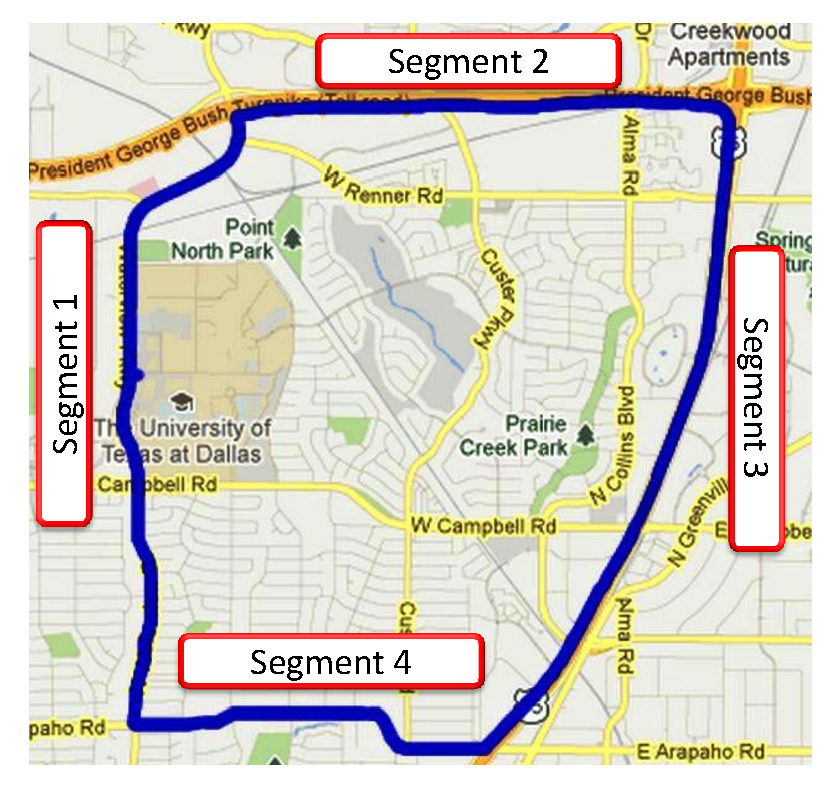
\includegraphics[width=0.6\linewidth]{figures/route_map-crop}
	\caption {Driving route with different conversational task segments.}
	\label{fig:ch6_map}
	%\vspace{-5mm}
\end{figure}

\begin{itemize}
	
	\item Segment 1: At the beginning, in order to “break the ice” the passengers will initiate a simple conversation by asking the driver questions about casual topics such as the weather (Other topics may be chosen).
	\item Segment 2: In this segment one of the passengers picks an object and the driver and the other passenger are supposed to guess the object using the hints provided to them. Whoever guesses first is the winner. This game is chosen to increase turn-taking and overlapping speech segments.
	\item Segment 3: A set of TIMIT sentences are played through a portable tablet and the driver is required to repeat each sentence before the next sentence is played.
	\item Segment 4: An argument is initiated by one of the passengers. This second conversation is more involved compared to that in segment 1. The difference here is that the driver’s opinion on a debatable topic is asked and based on his/her answer, the passengers take the other side and try to argue on the subject.
	Each of the tasks described above takes place on one of the legs in the route as labeled on the map in Figure~\ref{fig:ch6_map}.
	
\end{itemize}




\subsection{Experimental results}
An advantage of this experimental setup over previous studies~\cite{sathyanarayanaITSC2012, sathyanarayanaSAE2013,ESPA} is that both the in-vehicle speech data and the data required for maneuver recognition are recorded by the portable device. 
This results in a more concise and cost effective data acquisition platform.

Statistical information from the inertial measurement sensors such as accelerometer and gyroscope of the portable device were extracted on a per frame basis (once per second). 
Statistical information such as maximum lateral acceleration, mean of the vehicle speed, variance of yaw-gyroscope (refer to \cite{sathyanarayanaITSC2012} for a detailed list) form the dominant feature space used in training the maneuver specific models. 
Using Support Vector Machines (SVM), the maneuver segments are recognized and classified with a high average accuracy of over $90\%$. 
Once classified, driving performance is evaluated for each maneuver according to its class. 
Thresholds are appropriately set in the feature space to identify any abnormal or risky driving patters. 
Examples of the driving performance evaluation is shown in Figure~\ref{fig:ch6_driving_performance}. 
This figure compares a drivers performance on the same route with and without the stimulus of competitive conversations. 
The regions marked green are locations where the driver drove similar to his usual driving pattern. Yellow regions correspond to where the driver showed slight variations in the driving pattern. 
The red regions are locations where the driver executed an abnormal or risky maneuver. 
All regions concur with the visual and perceptual verification obtained by looking at the video from the data recordings. 

\begin{figure*}[h!]
	%\vspace{-5mm}
	\centering
	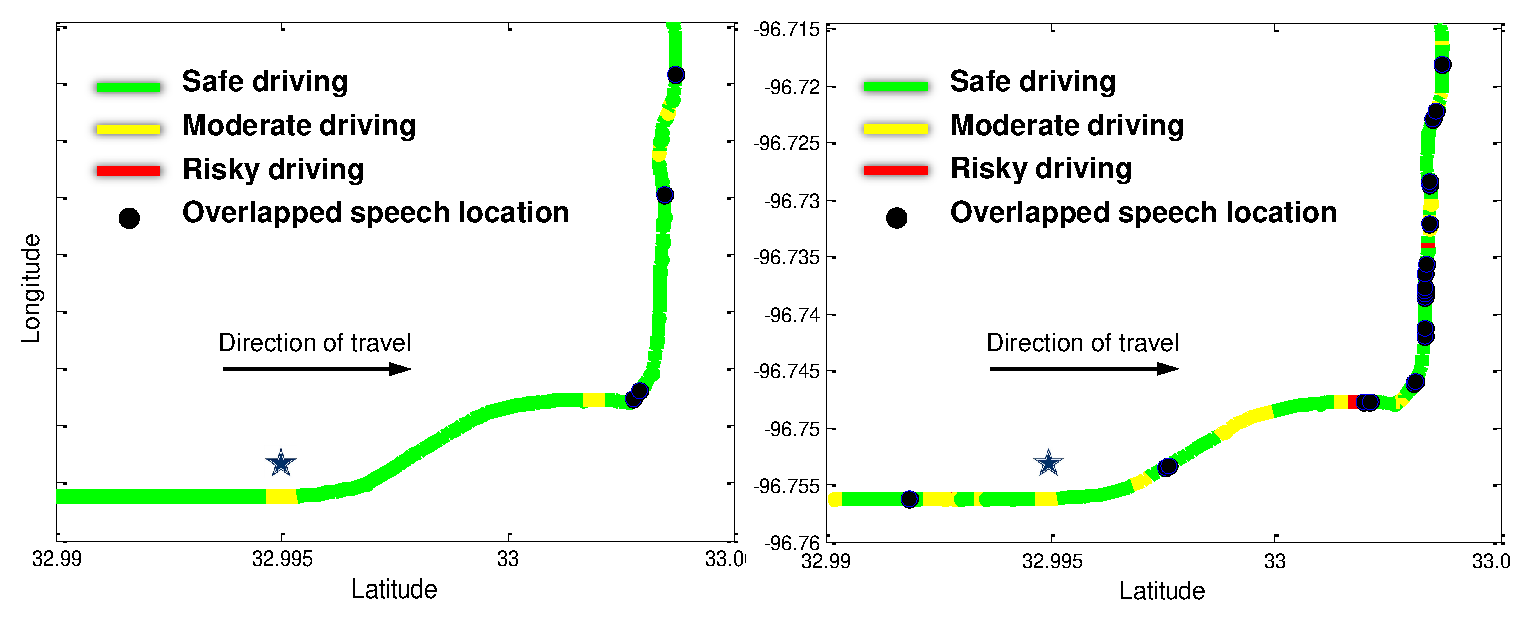
\includegraphics[scale=0.6]{figures/driving_and_overlap}
	\vspace{-5mm}
	\caption {Driving performance evaluation on a section of the route in two phases. Left (phase 1)-  performance with minimal conversations. Right (phase 2)- performance drop as a result of the increase in the amount of overlapping speech.}
	\label{fig:ch6_driving_performance}
	\vspace{-5mm}
	%\vspace{-5mm}
\end{figure*}


As Figure~\ref{fig:ch6_driving_performance} suggests, there are some instances in the route where no direct relationship is observed between overlapped speech and performance-drop, see the area marked by a star in the figure. 
This was expected, since there are always other sources that can cause irregularities in the driver's maneuver execution patterns. 
Hence, speech related features should be analyzed in more detail to confirm that the conversation is the source of distraction. 
With this intention, the patterns of turn-takings and overlapped speech segments were jointly investigated over time. 
Turn-taking and overlapped speech rates are defined as below:
\begin{equation}
ovl_{rate} = \dfrac{\textrm{Number\: of\: overlapped\: samples\: in\: window}}{\textrm{window\: length}} \nonumber
\end{equation}
\begin{equation}
tt_{rate} = \dfrac{\textrm{Number\: of\: turntakings\: in\: window}}{\textrm{window\: length}} \nonumber
\end{equation}

Figure~\ref{fig:ch6_turntaking_and_overlap} depicts the average turn-taking and overlapped speech rate in conversations before observing significant drop in driving performance. 
Each plot belongs to a different scenario. 

\begin{figure*}[h!]
	\vspace{1mm}
	\centering
	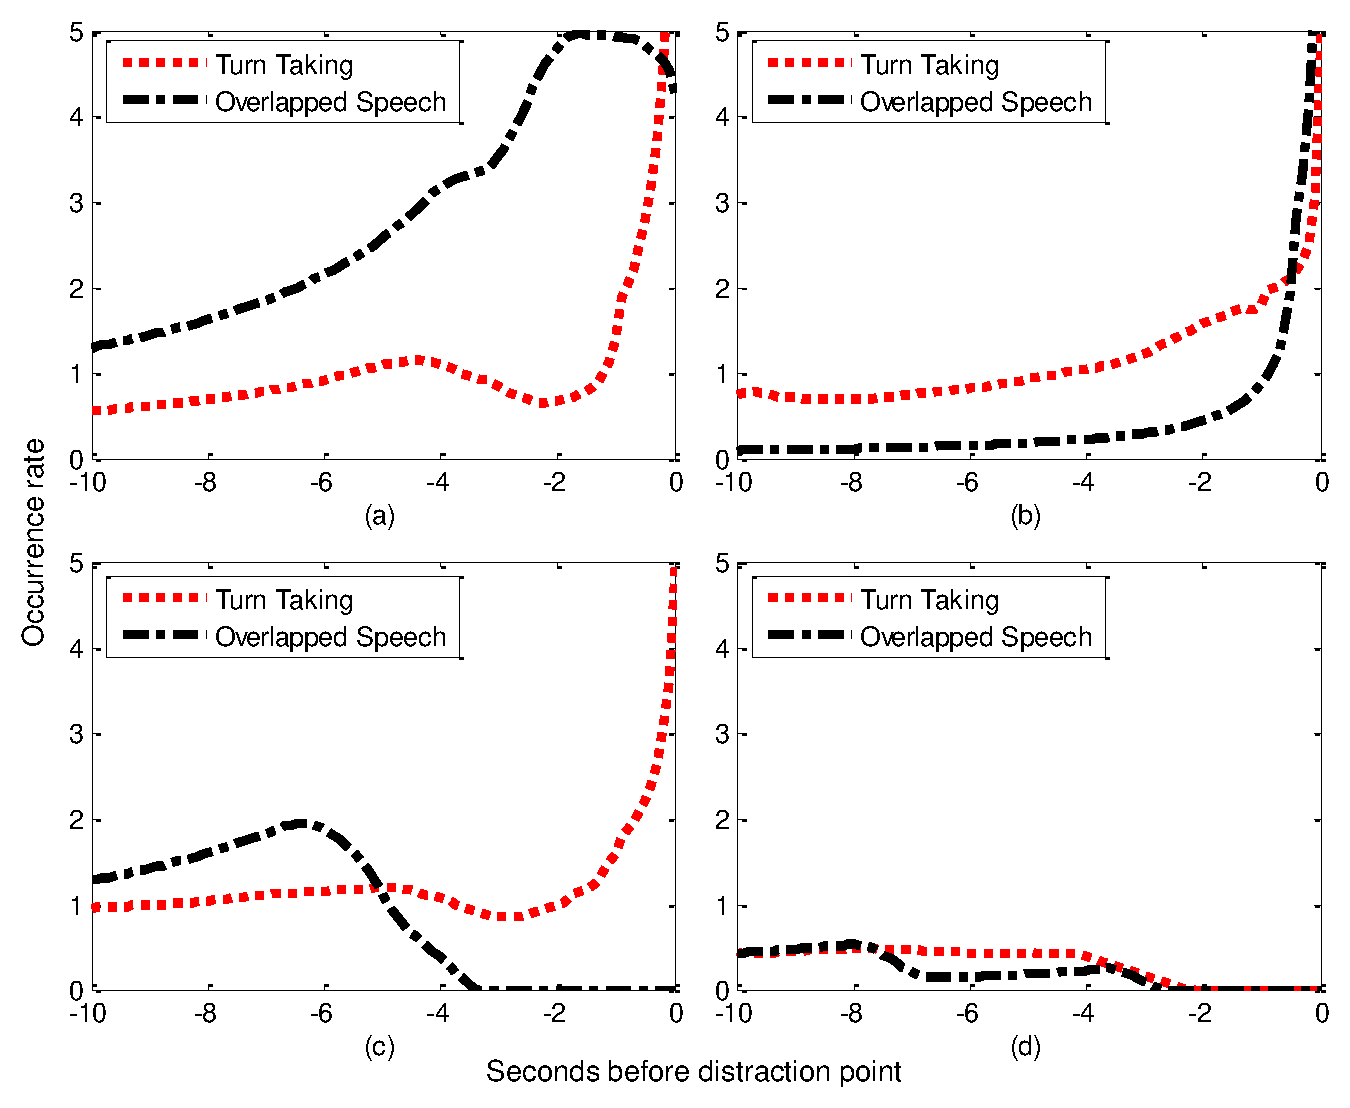
\includegraphics[scale=0.5]{figures/ttr_and_ovl}
	\caption {Turn-taking and overlapping speech rate before observing the first major drop in performance in different scenarios.}
	\label{fig:ch6_turntaking_and_overlap} 
	%\vspace{-5mm}
\end{figure*}

\newpage
If both the turn-taking and overlapped speech rates increase before the performance drops, the conversation can be a potential source of distraction. 
Figures~\ref{fig:ch6_turntaking_and_overlap}-a and b are more interesting, since both features increase with time. 
Figure~\ref{fig:ch6_turntaking_and_overlap}-c was also observed in our experiments, where the overlapped speech rate increases and goes back to $0$ per second before driving performance drops. 
Figure~\ref{fig:ch6_turntaking_and_overlap}-d shows an instance where turn-taking and overlapped speech rate significantly drop prior to any changes are observed in driving performance, lowering the possibility that the conversation being the source of distraction. 

\newpage
\section{Summary}
\label{sec:ch4_summary}
The final chapter highlights a selection of collaborative studies between co-channel speech analysis and other signal processing applications. 
The content was presented in the form of an applications chapter. 
The first section describes how overlap detection can be integrated into a word-count estimation system to reduce false-alarm errors in detecting syllables. 
The second section uses co-channel speech analysis, namely turn-taking rate estimation and overlap detection, to measure speakers' attentiveness in conversations. 
The predicted ``attentive'' is used in a driver safety system to identify in-vehicle conversations that jeopardize driver and passenger safety. 
